%%%%%%%%%%%%%%%%%%%%%%%%%%%%%%%%%%%%%%%%%%%%%%%%%%%%%%%%%%%%%%%%%%%%%%%%%%%%%%%%

\newcommand{\smin}{s_\text{min}}
\newcommand{\smax}{s_\text{max}}
\newcommand{\qhi}{q_\text{hi}}
\newcommand{\qlo}{q_\text{lo}}
\newcommand{\zero}{\text{\textbf{0}}}
\newcommand{\Zproj}{Z^{\textit{proj}}}
\newcommand{\Zowa}{Z^{\textit{owa}}}
\newcommand{\nowa}{n^{\textit{owa}}}
\newcommand{\Q}{\mathcal{Q}}
\newcommand{\Y}{\mathcal{Y}}
\newcommand{\X}{\mathcal{X}}
\newcommand{\matW}{\hat W}
\newcommand{\matV}{\hat V}
\newcommand{\W}{{\mathcal W}}
\newcommand{\Wowa}{{\hat \Theta^{\textit{owa}}}}
\newcommand{\Waff}{\mathcal{\hat A}}
\newcommand{\WaffE}{{\mathcal{\hat A}_\E}}
\newcommand{\Wave}{{\mathcal{\hat W}^{ave}}}
\newcommand{\Wtave}{{\mathcal{W}^{ave,*}}}
\newcommand{\V}{\mathcal{V}}
\newcommand{\A}{\mathcal{A}}
\newcommand{\D}{\mathcal{D}}
\newcommand{\E}{\mathbb{E}}
\newcommand{\vv}{\mathbf{v}}
\newcommand{\z}{\mathbf{z}}
\newcommand{\x}{\mathbf{x}}
\newcommand{\y}{\mathbf{y}}
\newcommand{\w}{\mathbf w}
\newcommand{\wkl}{\hat\w^{kl}}
\newcommand{\ahat}{\hat\alpha}
\newcommand{\astar}{\alpha^*}
\newcommand{\afull}{\ahat^{\textit{full}}}
\newcommand{\wowa}{\hat\w^{owa}}
\newcommand{\wowafull}{\hat\w^{\textit{owa,full}}}
\newcommand{\wowastar}{\hat\w^{\textit{owa,*}}}
\newcommand{\wave}{\hat\w^{ave}}
\newcommand{\wtave}{\E\hat\w^{ave}}
\newcommand{\waver}{\hat\w^{ave,r}}
\newcommand{\wboot}{\hat\w^{boot}}
\newcommand{\wmle}{\hat\w^{erm}}
\newcommand{\wmler}{\hat\w^{erm,r}}
\newcommand{\wstar}{{\w^{*}}}
\newcommand{\what}{{\hat\w}}
\newcommand{\wq}{\hat\w^{q}}
\newcommand{\wqstar}{\hat\w^{q^*}}
\newcommand{\reg}{r}
\newcommand{\loss}{\ell}
\newcommand{\Loss}{\mathcal{L}}

\newcommand{\trans}[1]{\ensuremath{{#1}^{\mathsf{T}}}}
\newcommand{\pinv}[1]{\ensuremath{{#1}^{\mathsf{\dagger}}}}
\newcommand{\ltwo}[1]{{\lVert {#1} \rVert}}
\newcommand{\ltwobig}[1]{{\left\lVert {#1} \right\rVert}}
\newcommand{\lone}[1]{{\lVert {#1} \rVert}_1}
\newcommand{\lzero}[1]{{\lVert {#1} \rVert}_0}
\newcommand{\proj}[1]{\pi_{{#1}}}
\newcommand{\prob}[1]{\Pr\left[{#1}\right]}

%%%%%%%%%%%%%%%%%%%%%%%%%%%%%%%%%%%%%%%%

\begin{frame}{Distributed ERM overview}

Overview
\begin{itemize}
\item
ERM is a general machine learning framework

\item
There is no known method for exactly merging two ERM estimators

\item
I provide a method that improves the guarantees of existing methods

\end{itemize}

\vspace{0.15in}
Stretch goal
\begin{itemize}
\item A better method for determining the regularization strength
\end{itemize}

\end{frame}

%%%%%%%%%%%%%%%%%%%%%%%%%%%%%%%%%%%%%%%%

\begin{frame}{What is empirical risk minimization (ERM)?}

Solve the following optimization
\begin{equation}
\wmle = \argmin_{\w} \sum_{(y,\x)\in Z} \loss(y;\trans\w\x) + \lambda\reg(\w)
\end{equation}
where
\begin{itemize}
\item $Z$ is a dataset with $mn$ points
\item $y\in\Y\subset\mathbb R$
\item $\x\in\X\subset\mathbb R^d$
\item $\w\in\W\subset\mathbb R^d$
\item $\loss$ is the (not necessarily convex) loss function
\item $\reg : \W\to\mathbb R$ is the regularization function
\end{itemize}

\vspace{0.15in}
\textbf{Theory:} the statistical error decays as $\ltwo{\wstar-\wmle} \le O(\sqrt{d/mn})$ where $\wstar$ is the optimal parameter in $\W$.
\end{frame}

%%%%%%%%%%%%%%%%%%%%%%%%%%%%%%%%%%%%%%%%

\begin{frame}{The averaging distributed estimator}

Procedure:

\begin{itemize}

\item Assign to each machine $i\in\{1...m\}$ a dataset $Z_i$ with $n$ datapoints

\item Each machine calculates the local ERM

\begin{equation}
\wmle_i = \argmin_{\w} \sum_{(y,\x)\in Z_i} \loss(y;\trans\w\x) + \lambda\reg(\w)
\end{equation}

\item A central server calculates the averaging estimator

\begin{equation}
\wave = \frac{1}{m}\sum_{i=1}^m \wmle_i
\end{equation}

\end{itemize}

\textbf{Theory:}

%\begin{itemize}

\begin{equation}
\ltwo{\wstar-\wave} \le 
\ltwo{\wstar-\E\wave} 
+
\ltwo{\E\wave-\wave} 
\end{equation}

\hspace{1.9in}
$O(\sqrt{d/n})$
\hspace{0.3in}
$O(\sqrt{d/mn})$

\end{frame}

%%%%%%%%%%%%%%%%%%%%%%%%%%%%%%%%%%%%%%%%

\begin{frame}
\frametitle{The \uncover<1-6>{full} optimal weighted average (OWA)}

\uncover<2-7>{
\vspace{0.1in}
On the first round,
\begin{itemize}
\item
calculate the $\wmle_i$ and communicate them to each other machine
\end{itemize} 
}

\uncover<3-7>{
\vspace{0.1in}
On the second round, 
\begin{itemize}
\item 
Let $\Wowa = \vecspan\{\wmle_i\}_{i=1}^m$\uncover<7>{, $Z^{owa}$ be a new dataset}
}

\uncover<4-7>{
\item Calculate
\begin{align}
\label{eq:afull}
\wowa{}^{\uncover<1-6>{,full}} &= \argmin_{\w\in\Wowa} \sum _{(\x,y)\in Z^{\textit{\uncover<7>{owa}}}} \loss\left(y,\trans\x\w \right)
+
\lambda \reg(\w)
\end{align}
}
\end{itemize}

%\vspace{0.1in}
Graphical Intuition
\begin{center}
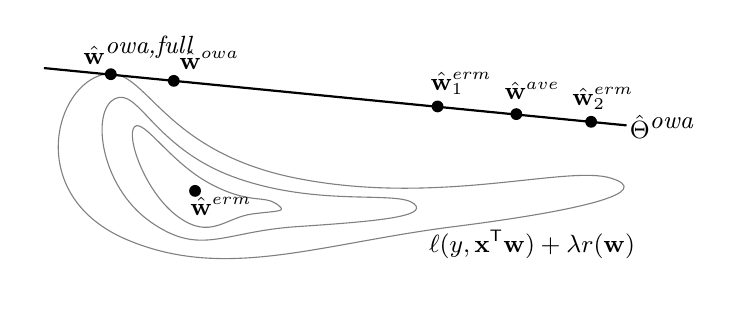
\begin{tikzpicture}
    [
    dot/.style = {minimum width=0.15cm,inner sep=0pt,line width=0pt,fill,circle,black,font=\small}
    , yscale=0.65
    ]
\small
\draw[gray] plot [smooth cycle,tension=1] coordinates {(-0.5,-0.75) (-1.05,1) (-0.1,-0.1) (0.75,-0.5) (0.45,-0.7) };
\draw[gray] plot [smooth cycle,tension=1] coordinates {(-0.85,-0.85) (-1.3,1.55) (0.25,0) (2.5,-0.5) (1,-0.95)};
\draw[gray] plot [smooth cycle,tension=1] coordinates {(-1.15,-1.2) (-1.5,2) (1,0) (5,0) (3,-0.95)};

\node[dot] (wstar) at (-0.28,-0.25) {};
\node at (0.05,-0.55) {$\wmle$};

\uncover<3-7>{
\draw[thick] (-2.2,2.15) -- (5.2,1.03);
\node at (5.65,1.0) {$\Wowa$};
}

\uncover<2-7>{
%\node[dot] (wstarproj) at (0.1,1.8) {};
%\draw (wstar) -- (wstarproj);
%\draw (0.07,1.65) -- (0.23,1.62) -- (0.26,1.78);

%\node[dot] (wavestar) at (4,0.5) {};
%\node                 at (4.5,0.3) {$\E\wave$};
\node[dot] (wave) at (2.80,1.40) {};
\node at (3.1,1.85) {$\wmle_1$};
\node[dot] (wave) at (4.75,1.10) {};
\node at (4.9,1.55) {$\wmle_2$};
%\node[dot] (wave) at (3.8,1.25) {};

}

\uncover<4-7>{
\node[dot] at (-1.35,2.03) {};
\node at (-1.0,2.5) {$\wowafull$};
}

\uncover<6-7>{
\node[dot] (wave) at (3.8,1.25) {};
\node at (4.0,1.7) {$\wave$};
}

\uncover<7>{
\node[dot] at (-0.55,1.9) {};
\node at (-0.1,2.3) {$\wowa$};
}

\node at (4,-1.3) {$\loss(y,\trans\x\w)+\lambda \reg(\w)$};
%\node at (6.95,1.0) {$\Wowa = \vecspan\{\wmle_i\}_{i=1}^m$};

\end{tikzpicture}
\end{center}

\end{frame}

%%%%%%%%%%%%%%%%%%%%%%%%%%%%%%%%%%%%%%%%

\begin{frame}{Efficiently calculating $\wowa$}

%Let $\matW = \bigg(\wmle_1, \wmle_2, ..., \wmle_m\bigg) \in \mathbb R^{d\times m}$
%
%\vspace{0.1in}
%Then every $\w\in\Wowa$ can be written as $\w=\matW\alpha$, where $\alpha\in\mathbb R^m$

\vspace{0.1in}
We can rewrite $\wowa$ as
%$\wowa = \matW \ahat$
%where
\begin{align}
\wowa &= \matW \ahat
\\
\label{eq:afull}
\ahat &= \argmax_{\alpha\in\mathbb R^m} \sum _{(\x,y)\in \Zowa} \loss\left(y,\trans\x \matW \alpha \right)
+
\lambda \reg(\matW\alpha)
\\
\matW &= \bigg(\wmle_1, \wmle_2, ..., \wmle_m\bigg) \in \mathbb R^{d\times m}
\end{align}

In the second round of communication
\begin{itemize}
\item Each machine transmits $\trans\x\matW$ for each data point in $\Zowa$
\item This is $O(m)$ bits per data point 

~~~~~~~~~$O(m\nowa)$ bits per machine

~~~~~~~~~$O(m^2\nowa)$ bits total
%\item Whenever $m\nowa < d$, fewer bits are transfered than the first round
\end{itemize}

\end{frame}

%%%%%%%%%%%%%%%%%%%%%%%%%%%%%%%%%%%%%%%%

\begin{frame}{Very little data is needed in the second optimization}

\vspace{0.15in}
\textbf{Theory:}
The dimension of the second optimization problem is $m$,

so $O(m) <\!\!< n$ data points are needed.

\vspace{0.15in}
\textbf{Experiment:}
Ad-click data with $m=128$, $mn=2.3\times10^8$, $d=7.4\times10^5$
%\vspace{0.15in}

\begin{center}
\begin{tabular}{cc}
\rotatebox{90}{\hspace{0.5cm}log-loss on held out data}
\hspace{0.1in}
&
\hspace{-0.5cm}
\begin{tikzpicture}
\node at (3.5,3.5) {\textcolor{darkgreen}{$\wowa$}};
\draw[->,darkgreen,very thick] (3.0,3.5) -- (2.5,3.5);

\node at (1,0.5) {\textcolor{red}{$\wboot$}};
\draw[->,red,thick] (0.6,0.7) -- (0.5,0.95);

\node at (1,2.1) {\textcolor{blue}{$\wave$}};
\draw[->,blue] (0.9,2) -- (1.0,1.75);

\begin{axis}
    [ width=4in
    , height=2.3in
    , xmin=1
    , xmax=1048576
    , ymin = 0.137
    , ymax = 0.14
    , y tick label style={
        /pgf/number format/.cd,
            fixed,
            fixed zerofill,
            precision=3,
        /tikz/.cd
    },
    , xtick={1,32,1024,32768,1048576}
    , log basis x={2}
    , xmode=log
    ]
%\addplot[blue,no marks] coordinates {(1,0.1376699823) (1048576,0.1376699823)};
%\addplot[thick,red,no marks] coordinates {(1,0.137198363008) (1048576,0.137198363008)};
%\addplot[very thick,darkgreen,no marks] table [x=nowa,y=128ll] {dat/kdd-nowa.dat};
\addplot[blue,no marks] coordinates {(1,0.138045477888) (1048576,0.138045477888)};
\addplot[thick,red,no marks] coordinates {(1,0.137682508908) (1048576,0.137682508908)};
\addplot[very thick,darkgreen,no marks] table [x=nowa,y=16ll] {dat/kdd-nowa.dat};
\end{axis}
\end{tikzpicture}
\\
&
\hspace{-0.15cm} data points used in second optimization $(\nowa)$
\end{tabular}
\end{center}

\end{frame}

%%%%%%%%%%%%%%%%%%%%%%%%%%%%%%%%%%%%%%%%

\begin{frame}{Scalability of OWA}
\textbf{Theory:}
The error scales as $\ltwo{\wmle-\wowa}\le O(\sqrt{1-(m/d)})$.

%\uncover<2>{
%\hspace{1.69in} $\E\ltwo{\wstar~~-\wowa}\le O(\sqrt{d/mn})$
%}

\vspace{0.15in}
\textbf{Experiment:}
%Same data as before with $\nowa=2^{10}$
Same data with $\nowa=2^{10}$, $mn=2.3\times10^8$, $d=7.4\times10^5$

\begin{center}
\begin{tabular}{cc}
\rotatebox{90}{\hspace{0.5cm}log-loss on held out data}
&
\hspace{-0.25cm}
\begin{tikzpicture}
\node at (5.3,1.35) {\textcolor{blue}{$\wave$}};
\draw[->,blue] (5.1,1.1) -- (5,0.9);
\node at (2.5,2.35) {\textcolor{red}{$\wboot$}};
\draw[->,red,thick] (2.2,2.1) -- (2,1.75);

\node at (1.0,0.85) {\textcolor{darkgreen}{$\wowa$}};
\draw[->,darkgreen, very thick] (1.0,1.2) -- (1.2,1.4);
\begin{axis}
    [ width=4in
    , height=2.3in
    , xmin=2
    , xmax=128
    , ymin = 0.137
    , ymax = 0.142
    , ytick={0.137,0.138,0.139,0.14,0.141,0.142}
    , y tick label style={
        /pgf/number format/.cd,
            fixed,
            fixed zerofill,
            precision=3,
        /tikz/.cd
    },
    %, xtick={2,4,128}
    , log basis x={2}
    , xmode=log
    ]
\addplot[blue,no marks] table [x=n,y=avell] {dat/kdd-scaling.dat};
\addplot[thick,red,no marks] table [x=n,y=bootll] {dat/kdd-scaling.dat};
\addplot[very thick,darkgreen,no marks] table [x=n,y=owall] {dat/kdd-scaling.dat};
\end{axis}
\end{tikzpicture}
\\
&
\hspace{0.5cm}number of machines ($m$)
\end{tabular}
\end{center}
\end{frame}


